%% ISAE-SUPAERO report template for research projects 
%% V1.0
%% 2016/04/14
%% by Damien Roque
%% See http://personnel.isae.fr/damien-roque


%% This template is based on bare_conf.tex
%% V1.4b
%% 2015/08/26
%% by Michael Shell

%%*************************************************************************
%% Legal Notice:
%% This code is offered as-is without any warranty either expressed or
%% implied; without even the implied warranty of MERCHANTABILITY or
%% FITNESS FOR A PARTICULAR PURPOSE! 
%% User assumes all risk.
%% In no event shall the IEEE or any contributor to this code be liable for
%% any damages or losses, including, but not limited to, incidental,
%% consequential, or any other damages, resulting from the use or misuse
%% of any information contained here.
%%
%% All comments are the opinions of their respective authors and are not
%% necessarily endorsed by the IEEE.
%%
%% This work is distributed under the LaTeX Project Public License (LPPL)
%% ( http://www.latex-project.org/ ) version 1.3, and may be freely used,
%% distributed and modified. A copy of the LPPL, version 1.3, is included
%% in the base LaTeX documentation of all distributions of LaTeX released
%% 2003/12/01 or later.
%% Retain all contribution notices and credits.
%% ** Modified files should be clearly indicated as such, including  **
%% ** renaming them and changing author support contact information. **
%%*************************************************************************

\documentclass[conference]{IEEEtran}

\usepackage[utf8]{inputenc}
\usepackage{ifthen}
\usepackage{cite}
\usepackage[pdftex]{graphicx}
\graphicspath{{images/}}
\usepackage{tikz,filecontents}
\usetikzlibrary{shapes,arrows,shadings,patterns}
\usepackage{pgfplots}
\pgfplotsset{compat=newest}
\pgfplotsset{plot coordinates/math parser=false}
\newlength\figureheight
\newlength\figurewidth

\usepackage{amsfonts}
\usepackage[cmex10]{amsmath}
\usepackage{multirow}
\documentclass[a4paper,12pt]{article}
\usepackage[english]{babel}
\usepackage[latin1]{inputenc}
\usepackage[usenames]{color}




% Examples of several macros
\newcommand*{\SET}[1]{\ensuremath{\boldsymbol{#1}}}
\newcommand*{\VEC}[1]{\ensuremath{\boldsymbol{\mathrm{#1}}}}
\newcommand*{\FAM}[1]{\ensuremath{\mathrm{#1}}}
\newcommand*{\MAT}[1]{\ensuremath{\boldsymbol{\mathrm{#1}}}}
\newcommand*{\OP}[1]{\ensuremath{\mathrm{#1}}}
\newcommand*{\NORM}[1]{\ensuremath{\left\|#1\right\|}}
\newcommand*{\DPR}[2]{\ensuremath{\left \langle #1,#2 \right \rangle}}

\newtheorem{theorem}{Theorem}

\newcommand{\alert}[1]{\textcolor{red}{#1}}
\usepackage[caption=false,font=footnotesize]{subfig}
\usepackage{url}


% correct bad hyphenation here
\hyphenation{op-tical net-works semi-conduc-tor}


\begin{document}
%
% paper title
% Titles are generally capitalized except for words such as a, an, and, as,
% at, but, by, for, in, nor, of, on, or, the, to and up, which are usually
% not capitalized unless they are the first or last word of the title.
% Linebreaks \\ can be used within to get better formatting as desired.
% Do not put math or special symbols in the title.
\title{Flutter sensibility to semi-aeroelastic hinged wing parameters}

% for over three affiliations, or if they all won't fit within the width
% of the page, use this alternative format:
% 
\author{\IEEEauthorblockN{Carlos Nicol\'as Juarez\IEEEauthorrefmark{1},
Joseph Morlier\IEEEauthorrefmark{2}}
\IEEEauthorblockA{\IEEEauthorrefmark{1}Institut Supérieur de l'Aéronautique et de l'Espace (ISAE-SUPAERO), Université de Toulouse, 31055 Toulouse, FRANCE\\
Email: carlos.juarez@student.isae-supaero.fr}
\IEEEauthorblockA{\IEEEauthorrefmark{2}Institut Supérieur de l'Aéronautique et de l'Espace (ISAE-SUPAERO), Université de Toulouse, 31055 Toulouse, FRANCE\\
Email: joseph.morlier@isae-supaero.fr}
}


%\IEEEspecialpapernotice{(Bibliography report)}
\IEEEspecialpapernotice{(Final report)}


% make the title area
\maketitle

% As a general rule, do not put math, special symbols or citations
% in the abstract


\begin{abstract}
The benefits of high aspect ratio wings in lift-induced drag are well known. However, this solution has well-defined limits imposed by airport regulation and increasing loads. The introduction of a hinged wingtip is a possible solution for both problems. The aim of this research is to study the influence of hinge parameters on the flutter performance of the wing.
\end{abstract}

\IEEEpeerreviewmaketitle

\section*{Nomenclature}
\subsection*{Symbols}
\begin{tabular}{l l}
$k_{hinge}$&    Hinge stiffness\\
$y_{hinge}$&    Hinge position\\
$\Lambda$&      Flare angle\\
$\theta$ &      Winglet rotation angle\\
$M_{hinge}$&    Hinge moment\\
$\textbf{q}$&   Modal amplitudes\\
$\textbf{M}$&   Mass matrix\\
$\textbf{C}$&   Damping matrix\\
$\textbf{K}$&   Stiffness matrix\\
$q_{\infty}$&   Dynamic pressure\\
$V_f$&          Flutter speed\\
\end{tabular}

\subsection*{Abbreviations}

\begin{tabular}{l l}
HAR&    High aspect ratio\\
SAH&    Semi-aeroelastic hinge\\
DLM&    Doublet lattice method\\
WRBM&   Wing root bending moment\\
MAC&    Mean aerodynamic chord\\
HTP&    Horizontal tail plane\\
VTP&    Vertical tail plane\\
GUI&    Graphic user interface\\
DoF&    Degrees of freedom\\
\end{tabular}



\section{Introduction}
\label{sec:problem-statement}

One of the most efficient strategies to reduce aerodynamic drag is to attack the lift-induced drag given that it contributes approximately 40\% of the overall drag. Induced drag is created at the tips of the wings where the high pressure air from beneath the wing comes up over the wing tips into the low pressure zone. This meeting place of different air pressures becomes a turbulent area creating induced drag. High aspect ratio (HAR) wings reduce considerably this effect, since the lift-induced drag is proportional to the reciprocal of the wingspan squared. Despite this great advantage, HAR wings are limited by two main issues: On one hand, maximum aircraft dimensions allowed in airports, and on the other hand the increase in bending moments along the wing.

In the last years, some attempts were made in order to increase civil aircraft wingspan; for example, the implementation of a folding wingtip in the Boeing 777X which enables the reduction of the wingspan when grounded in order to respect airport regulations.

In this research, an alternative design is studied, which is a potential solution for both problems mentioned. The main idea consists in introducing a hinge (with a certain stiffness) in order to allow the wing tips to rotate as can be seen in fig. \ref{fig:HingedWing}. Such a concept is called semi-aeroelastic hinge (SAH) \cite{Castrichini2016,Castrichini2020}. 

\begin{figure}[htp]
  \centering
  \setlength\figureheight{5cm}
  \setlength\figurewidth{6cm}
  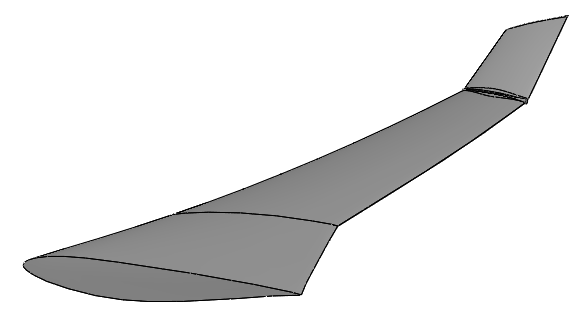
\includegraphics[width=200pt]{images/HingedWing.png}
  \caption{Geometric model of a SAH}
  \label{fig:HingedWing}
\end{figure}

Significant progress in this field is the Airbus project AlbatrosONE, which consists of a small scale demonstrator, and, so far, has presented optimistic results from wind tunnel tests and from the first flight tests \cite{wilson2019small}.

This solution has shown itself to be quite favourable when looking for load alleviation. Previous studies found between 10\% and 20\% reduction in the wing root bending moment (WRBM) depending on the design chosen and the conditions studied. Despite these benefits, the hinge presence may introduce instabilities to the aircraft, generating undesired effects like flutter.

This research looks to analyse flutter, which is a dangerous aeroelastic phenomenon that arises from an unfavourable coupling between aerodynamic, elastic and inertial forces. This instability produces large displacements that can generate severe damage or even destruction of the aircraft and hence, it must be taken into account from a preliminary design phase. The idea in this work is to better understand how flutter is affected by hinge parameters.


\section{Problem statement}
\label{sec:problem-statement}

The aim of this work is to represent this new design solution by using low-fidelity models and then to modify the main parameters concerning the hinge in order to see how they affect flutter speed.

The framework to be used for this work is NeoCASS, a free suite of Matlab modules that combines state of the art computational, analytical and semi-empirical methods to run aero-structural analysis of a design layout at conceptual design stage. It works with NASTRAN derived formats \cite{cavagna2011neocass}.

One of the challenges that arise in order to work with this framework is that even if non-conventional designs are supported, there is no option to model a semi-rigid hinge, therefore, a modification in the modelling process is needed to include it.

Several combinations of the hinge parameters will be done, computing flutter speed for each case in order to extract valuable information about its sensibility. An appropriate range of values will be defined for each parameters taking into account possible design solutions.

The idea is to choose those parameters that are most related to the hinge presence.

It is known that the hinge stiffness $k_{hinge}$ is a significant parameter. Previous works \cite{Wilson2014,Castrichini2016}show that a zero stiffness hinge is highly effective for load alleviation. However, this may generate instability and flutter.

Another important parameter is the hinge position $y_{hinge}$. Previous results indicate that moving the hinge inboard may produce a strong stabilising effect on the flutter mechanisms \cite{Wilson2014}.

Finally the orientation of the hinge line relative to the airflow (flare angle $\Lambda$) is a key parameter to enable successful load alleviation. When the hinge line is rotated outboard of the streamline, folding the wingtip up introduces a decrease in the local angle of attack; such an effect provides a means to reduce the loads acting on the wing, leading to the possibility of achieving a wing tip extension with limited or even minimal impact on wing weight \cite{Castrichini2020,Wilson2014}. Although this angle may also have an effect over the flutter speed this parameter will not be considered due to model limitations.


\section{Aeroelastic model}
\label{sec:aeroelastic-model}
A low-fidelity model is used in order to obtain results without high computational cost but still accurate enough to obtain qualitative information. The main modelling is done in AcBuilder \cite{acbuilderfurther}, a graphical editor where a conceptual design of the aircraft is done and also, the XML file requested by NeoCASS is generated.

\subsection{Aircraft modelling}
A long-range aircraft was used, based on the Boeing 747-100 which is already available as an example in NeoCASS. Therefore, only the hinge modelling was needed. Main geometric specification values are shown in table \ref{tab:GeoSpec}.

\begin{table}[t]
\begin{center}
\begin{tabular}{| l | r |}
\hline
Overall length & $68.5 \; m$ \\ \hline
Wing span & $59.64 \;m$ \\ \hline
Wing surface & $551 \;m^2$ \\\hline
MAC & $ \;10.0695 m$\\\hline
Airfoil &  N64A410\\ \hline
HTP surface & $135 m^2$\\\hline
VTP surface & $77.11 m^2$\\
\hline 
\end{tabular}
\caption{Geometric specifications}
\label{tab:GeoSpec}
\end{center}
\end{table}

The aircraft model as displayed in AcBuilder graphic user interface (GUI) is shown in figure \ref{fig:AircraftModel}.

\begin{figure}[htp]
  \centering
  \setlength\figureheight{5cm}
  \setlength\figurewidth{7cm}
  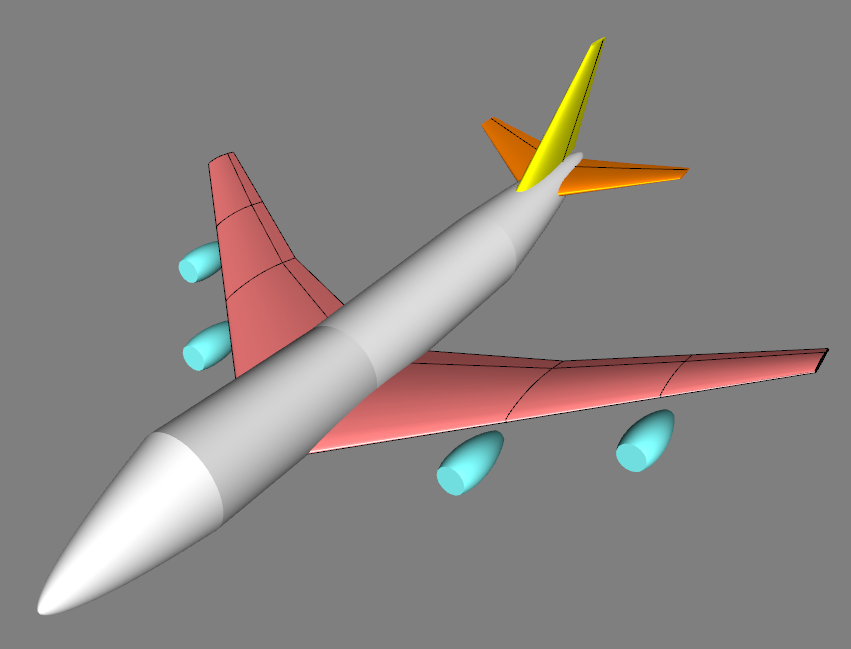
\includegraphics[width=225pt]{images/AircraftModel.png}
  \caption{Aircraft model}
  \label{fig:AircraftModel}
\end{figure}

\subsection{Structural modelling}
The structure was modelled using linear beam elements, discretizing each semi wing in $15$ elements. As a hinge definition is not supported by the AdBuilder GUI, a modification in the geometric file was needed. Thus the hinge was modelled by constraining two coincident nodes, one belonging to the main airframe and the other to the wing-tip, to have the same translations but free to have different relative rotations with respect to the hinge axis. This was done using CELAS, which is a zero-length Nastran elements used to model springs.

The implementation of CELAS elements is shown in figure \ref{fig:NastranHinge}, where a certain stiffness (in this case $k_{hinge} = 1e6 \frac{Nm}{rad}$) is given to the hinge rotation axis while the rest of the DoF are constrained with high stiffness values. In the figure example the spring element connect node $2015$ with node $2015555$ which is an intermediate node between nodes $2015$ and $2016$ and it is coincident with node $2015$.

\begin{figure}[htp]
  \centering
  \setlength\figureheight{5cm}
  \setlength\figurewidth{7cm}
  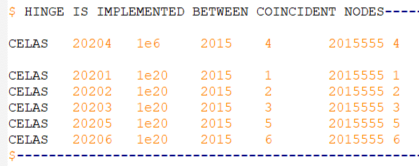
\includegraphics[width=225pt]{images/NastranHinge.png}
  \caption{CELAS elements implementation}
  \label{fig:NastranHinge}
\end{figure}

Previous works have shown that the wingtip mass has a certain influence in the flutter performance \cite{Castrichini2016}. In fact, for values lower than 300 kg, the sensitivity of the flutter speed with respect to the spring stiffness was negligible. Therefore, in order to analyze the hinge stiffness influence, concentrated masses were added to the wingtips using CONM2 Nastran elements. Their implementation is shown in figure \ref{fig:NastranCONM2}.

\begin{figure}[htp]
  \centering
  \setlength\figureheight{5cm}
  \setlength\figurewidth{7cm}
  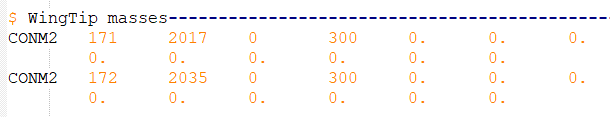
\includegraphics[width=225pt]{images/NastranCONM2.png}
  \caption{CONM2 elements implementation}
  \label{fig:NastranCONM2}
\end{figure}

The structural model and discretization is shown in figure \ref{fig:StructuralModel}.

\begin{figure}[htp]
  \centering
  \setlength\figureheight{5cm}
  \setlength\figurewidth{7cm}
  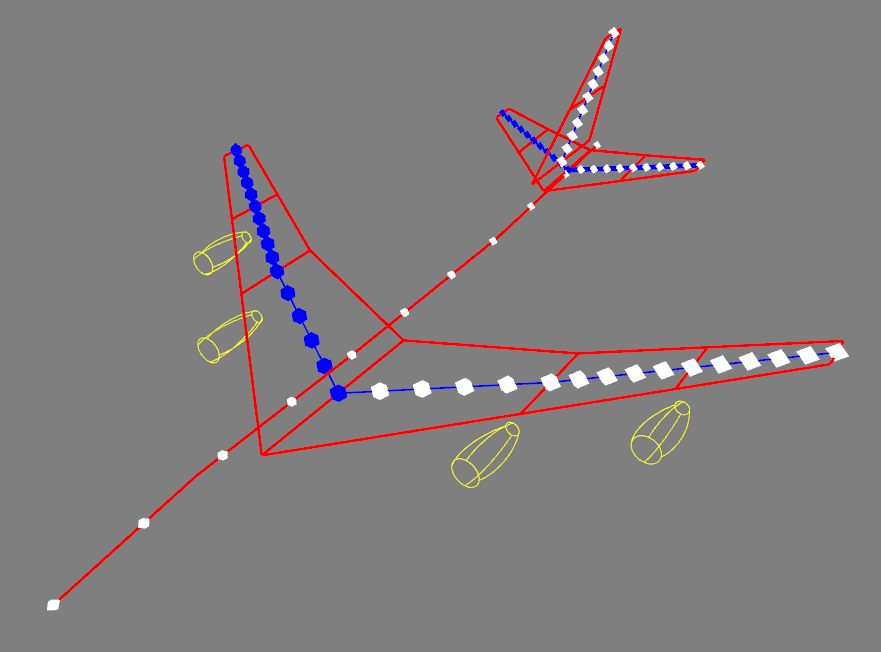
\includegraphics[width=225pt]{images/StructuralModel.png}
  \caption{Structural model}
  \label{fig:StructuralModel}
\end{figure}

Another important point to mention is that this aircraft has shown to be very resistant to aeroelastic instabilities. Therefore, Young's modulus of the wing beam elements was reduced by 10\% in order to evidence flutter effect and to be able to draw qualitative conclusions from it.

\subsection{Aerodynamic modelling}
In order to compute the unsteady loads that are needed for the flutter computation NeoCASS applies the Doublet lattice method (DLM). This is a method based on aerodynamic potential theory, where each of the interfering surfaces is divided into small trapezoidal lifting elements (panels) such that they are arranged in strips parallel to the free stream with surface edges, fold lines, and hinge lines lying on panel boundaries. The unknown lifting pressures are assumed to be concentrated uniformly across the one-quarter chord line of each panel. There is one control point per panel, centred span-wise on the three-quarter chord line of the panel, and the surface boundary condition is satisfied at each of these points.

The implemented aerodynamic model has 14 span-wise divisions and 7 chord-wise divisions and it is shown in figure \ref{fig:AeroModel}.

\begin{figure}[htp]
  \centering
  \setlength\figureheight{5cm}
  \setlength\figurewidth{7cm}
  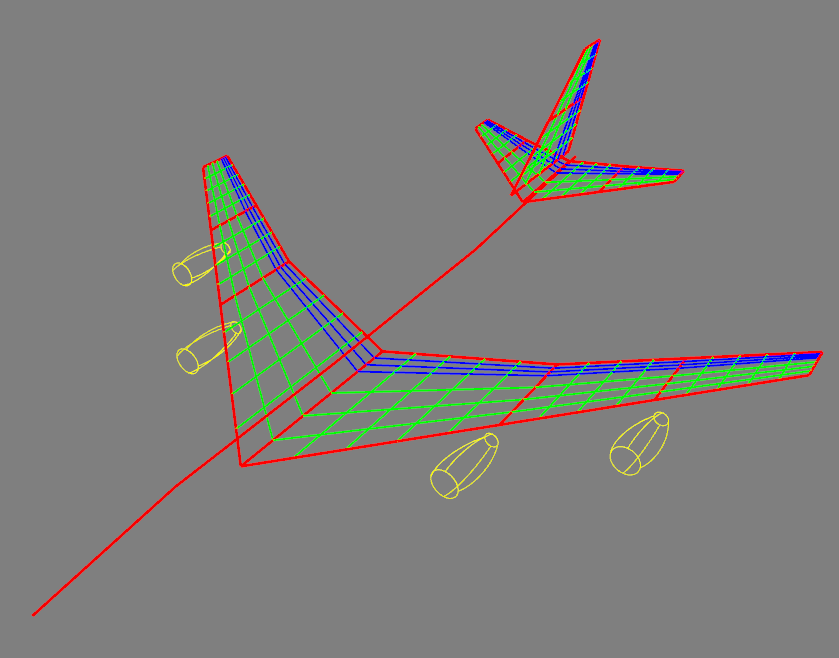
\includegraphics[width=225pt]{images/AeroModel.png}
  \caption{Aerodynamic model}
  \label{fig:AeroModel}
\end{figure}


\section{Analyzed parameters}

In order to understand the hinge behaviour, two of the main parameters related to its presence were considered: the hinge stiffness and the hinge position.

\subsection{Hinge stiffness}
The hinge is modelled as a rotational spring, which has a certain stiffness called $k_{hinge}$. When the winglet is deflected, the spring produces a moment proportional to the angle of rotation $\theta$:

\begin{equation}
    M_{hinge} = k_{hinge}[\frac{Nm}{rad}] \times \theta
\end{equation}

Based on previous works, the chosen stiffness values go from $k_{hinge} = 1e4 \;[Nm/rad]$ to $k_{hinge} = 1e10 \;[Nm/rad]$.

\subsection{Hinge position}
The hinge position is defined as the ratio between the coordinate of the node where the hinge is placed and the wing span. The range of  selected values for this analysis is the following:

\begin{itemize}
    \item $y_{hinge} = 0.67$
    \item $y_{hinge} = 0.72$
    \item $y_{hinge} = 0.78$
    \item $y_{hinge} = 0.83$
    \item $y_{hinge} = 0.89$
\end{itemize}

The identification of these nodes in the Nastran geometric file can be seen in figure \ref{fig:HingeRange}.

\begin{figure}[htp]
  \centering
  \setlength\figureheight{5cm}
  \setlength\figurewidth{6cm}
  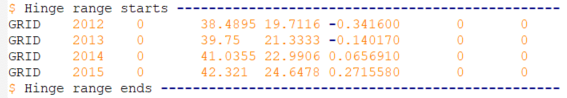
\includegraphics[width=250pt]{images/HingeRange.png}
  \caption{Hinge range in the geometric file}
  \label{fig:HingeRange}
\end{figure}


\section{Modal analysis}
Modal analysis, or the mode-superposition method, is a linear dynamic-response procedure which evaluates and superimposes free-vibration mode shapes to characterize displacement patterns. The purpose of a modal analysis is to find the shapes and frequencies at which the structure will amplify the effect of a load.

In order to compute flutter, modal analysis is needed for each hinge configuration. In the NeoCASS GUI this analysis can be easily set up.

For this work 20 modes were computed, where the first 6 modes correspond to the rigid modes of the plane. The range of frequencies is set up from $0\;[Hz]$ to $50\;[Hz]$ which is large enough to include the first 20 modes. The configuration of the analysis in the NeoCASS GUI is shown in figure \ref{fig:ModalGUI}.

\begin{figure}[htp]
  \centering
  \setlength\figureheight{5cm}
  \setlength\figurewidth{6cm}
  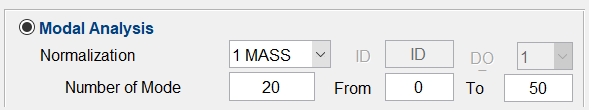
\includegraphics[width=250pt]{images/ModalGUI.png}
  \caption{Modal analysis set up}
  \label{fig:ModalGUI}
\end{figure}


\section{Flutter analysis}
\label{sec:flutter-analysis}
The flutter analysis technique implemented in NeoCASS is based on a well-consolidated continuation form.
Adopting the classic assumptions based on assumed structural shapes, the availability of an aerodynamic
transfer matrix $\textbf{H}_{am}$ and the Laplace domain $s$, the flutter problem reads\cite{cavagna2011aeroelastic}:

\begin{equation}
    (s^2 \textbf{M} + s \textbf{C} + \textbf{K} - q_{\infty} \textbf{H}_{am}(p,M_\infty))\textbf{q}=\textbf{0}
\end{equation}

Where $\textbf{q}$, $\textbf{M}$, $\textbf{C}$, $\textbf{K}$ are respectively modal amplitudes, mass, damping, and stiffness matrices, and $q_\infty$ is the dynamic pressure. Eq.(2) represents a complex eigenvalue problem and the method adopted for the solution is the one proposed in \cite{cardani1978continuation}.

For all the different combinations of the studied parameters the Mach number was fixed to $M = 0.84$. And the density was fixed to $\rho = 0.458 [\frac{kg}{m^3}]$ which is equivalent to an altitude of $30000\;ft$. These values were chosen in order to represent cruise conditions.

The 20 computed modes were considered for the modal base and all 14 non-rigid modes were considered for the flutter tracking.

With respect to the reduced frequencies, eight values were chosen as they can be seen in figure \ref{fig:redFreq}.

\begin{figure}[htp]
  \centering
  \setlength\figureheight{5cm}
  \setlength\figurewidth{6cm}
  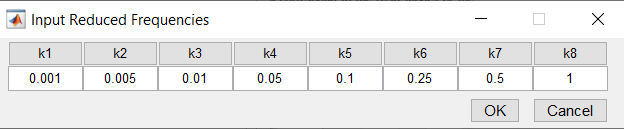
\includegraphics[width=250pt]{images/ReducedFreqGUI.png}
  \caption{Modal analysis set up}
  \label{fig:redFreq}
\end{figure}

In order to obtain results for a large amount of hinge stiffness values, a Matlab file was coded, where all the required stiffnesses are introduced as an array and then, the flutter analysis is run for each one of them. In order to do that, before each analysis, the code search in the structural file, the line where the hinge stiffness is defined (i.e. CELAS element rotation stiffness around "x" axis) and replaces it for the current value.

Finally, after each analysis, the flutter speed, as well as the unstable mode for each case are stored in array variables.

In figure \ref{fig:MatlabCode} the main loop of the described code is shown.

\begin{figure}[htp]
  \centering
  \setlength\figureheight{5cm}
  \setlength\figurewidth{6cm}
  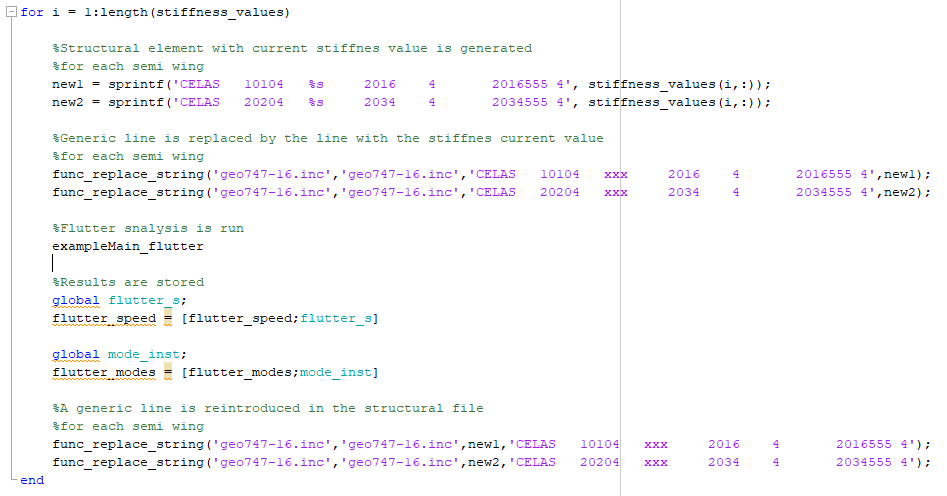
\includegraphics[width=250pt]{images/MatlabCode.png}
  \caption{Matlab code that manages the flutter analysis}
  \label{fig:MatlabCode}
\end{figure}


\section{Modal Results}

In figure \ref{fig:non-rigid modes}, the first four non-rigid modes can be seen for the case where the hinge is located at 78\% of the semi wing and the hinge stiffness is $k_{hinge} = 1e5 [Nm/rad]$. 


\begin{figure*}
\centering
\subfloat[Mode 7]{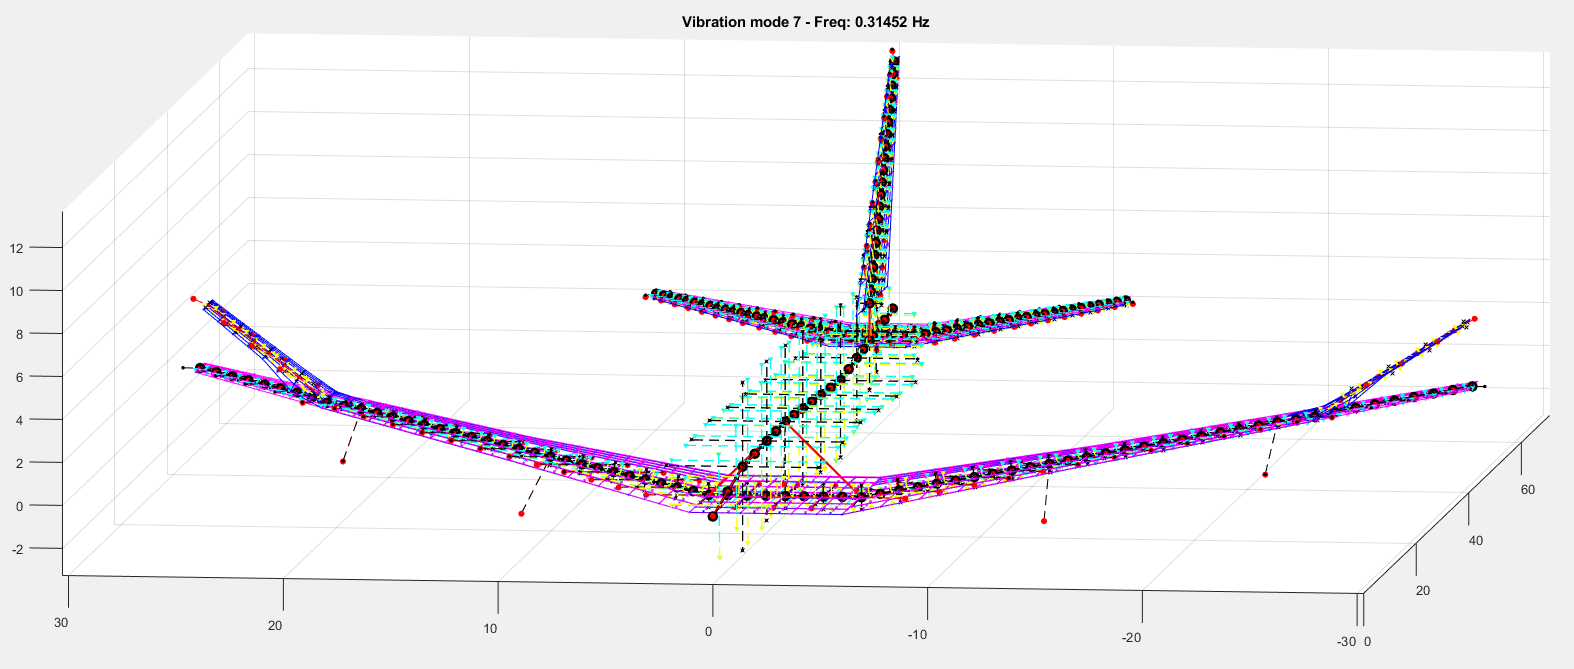
\includegraphics[width = 3in]{images/mode7.png}}\:\:\: 
\subfloat[Mode 8]{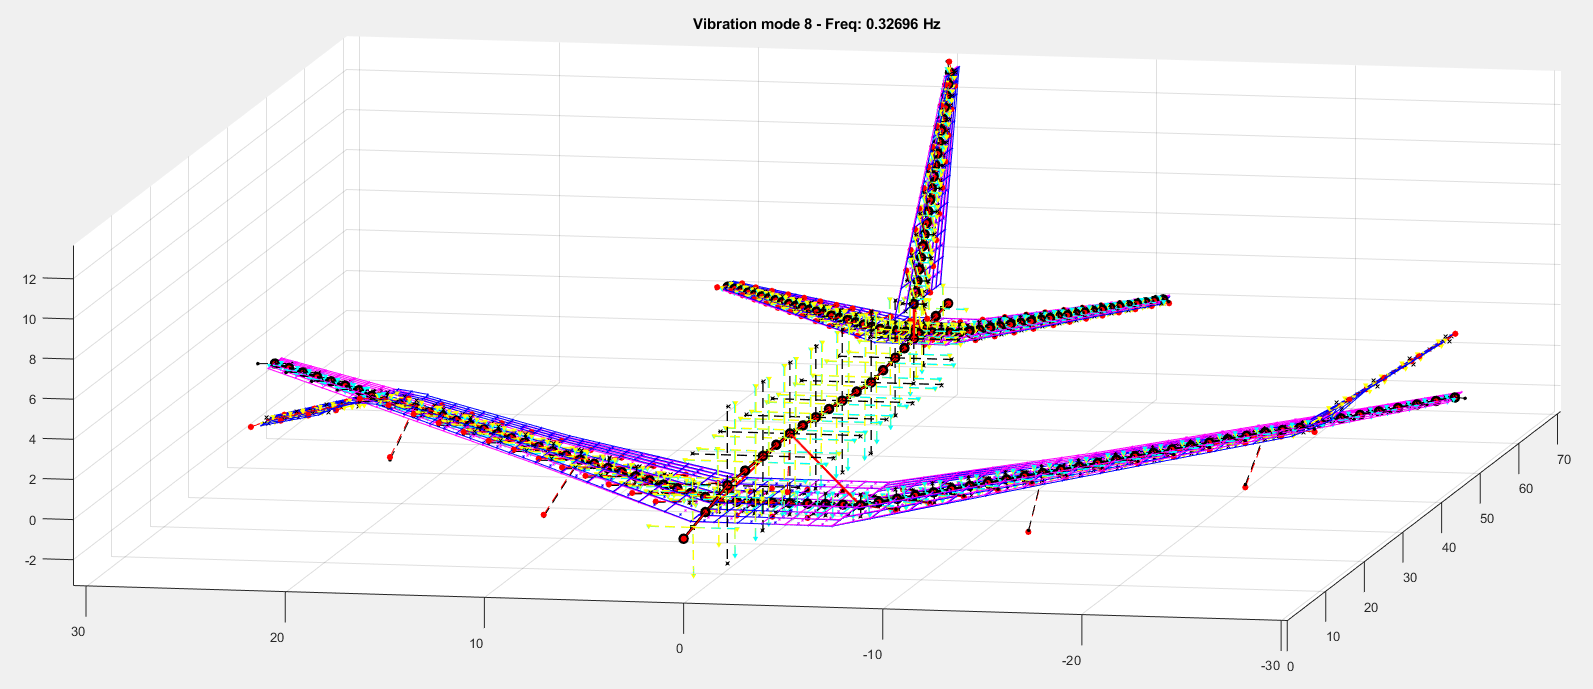
\includegraphics[width = 3in]{images/mode8.png}}\\
\subfloat[Mode 9]{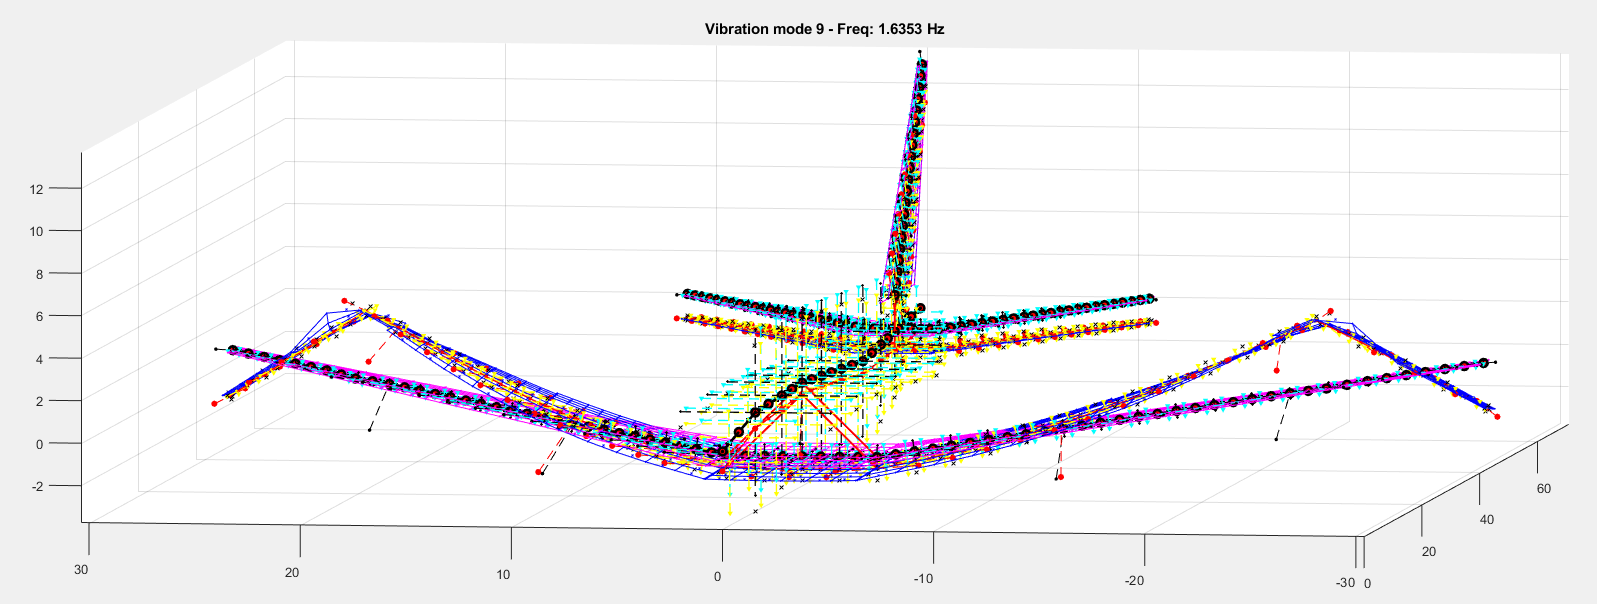
\includegraphics[width = 3in]{images/mode9.png}}\:\:\: 
\subfloat[Mode 10]{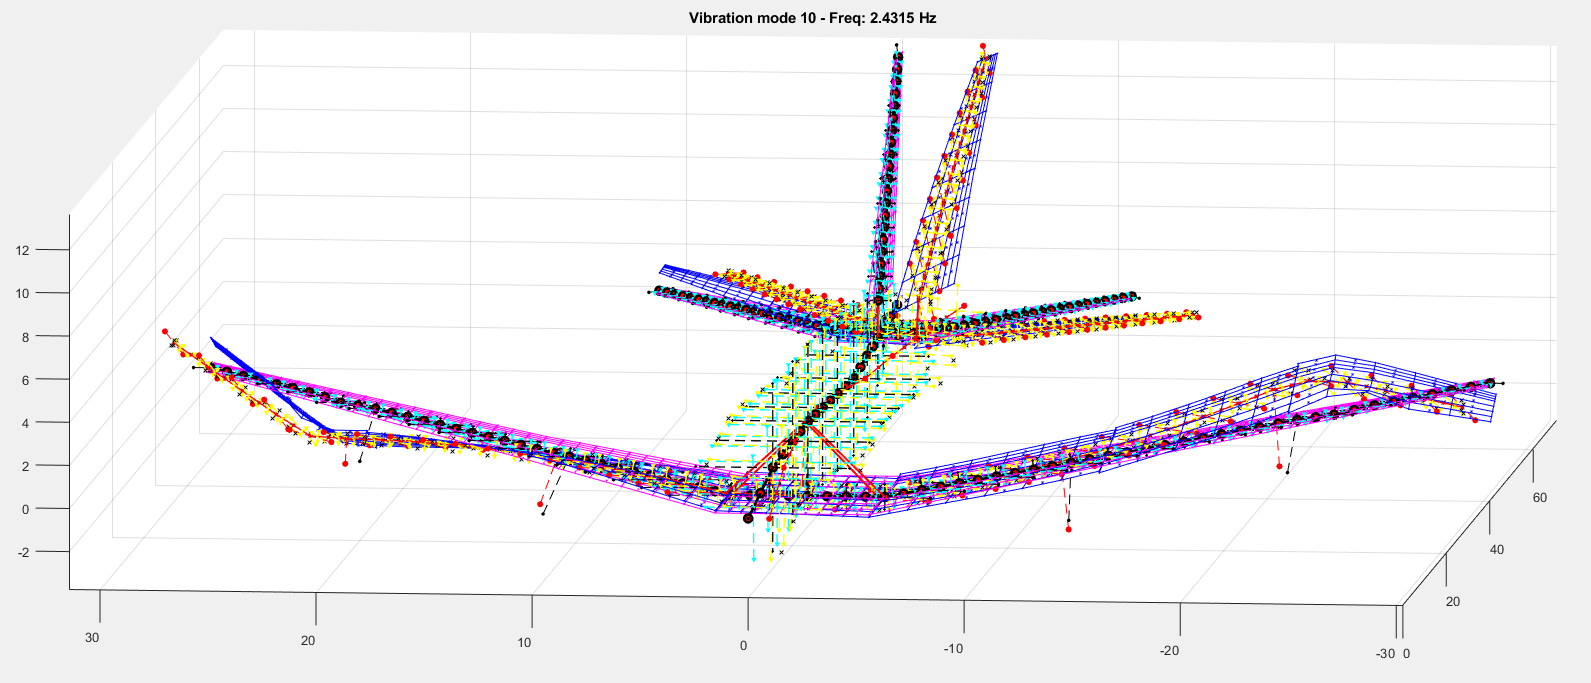
\includegraphics[width = 3in]{images/mode10.png}} 
\caption{First non-rigid modes - $k_{hinge} = 1e5$}
\label{fig:non-rigid modes}
\end{figure*}


The analysis showed that the first two non-rigid modes are wingtip modes since the only deflections are the symmetric and anti-symmetric wingtip rotations.

The remaining modes, including modes 9 and 10 shown in figure \ref{fig:non-rigid modes}, involve a combination of wingtip and main airframe deformations.

Another significant result arises when we compare wingtip modes (modes 7 and 8) between different hinge stiffness cases. In figure \ref{fig:modes7-8-1e8} the first two non-rigid modes are shown for the case where the hinge stiffnes is $k_{hinge} = 1e8 [Nm/rad]$.

\begin{figure*}
\centering
\subfloat[Mode 7]{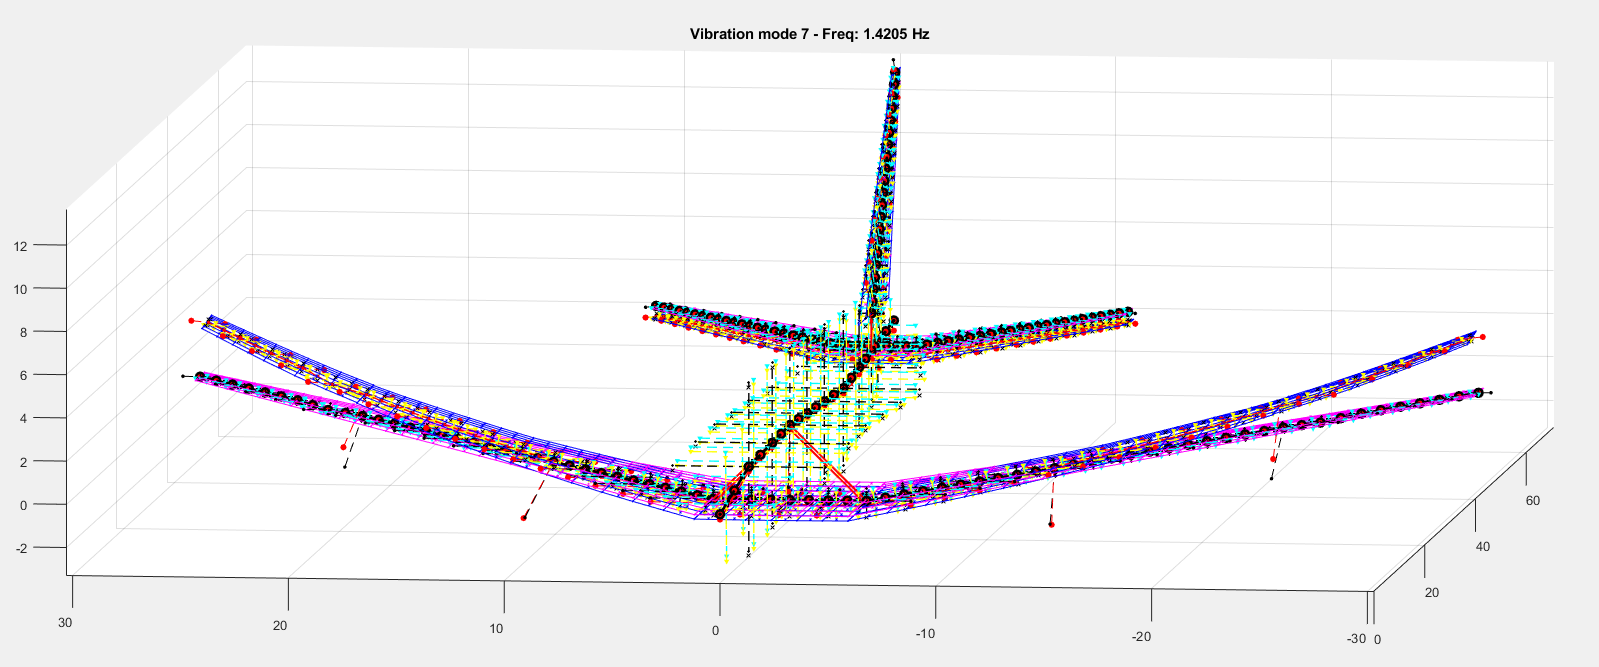
\includegraphics[width = 3in]{images/mode7-1e8.png}}\:\:\: 
\subfloat[Mode 8]{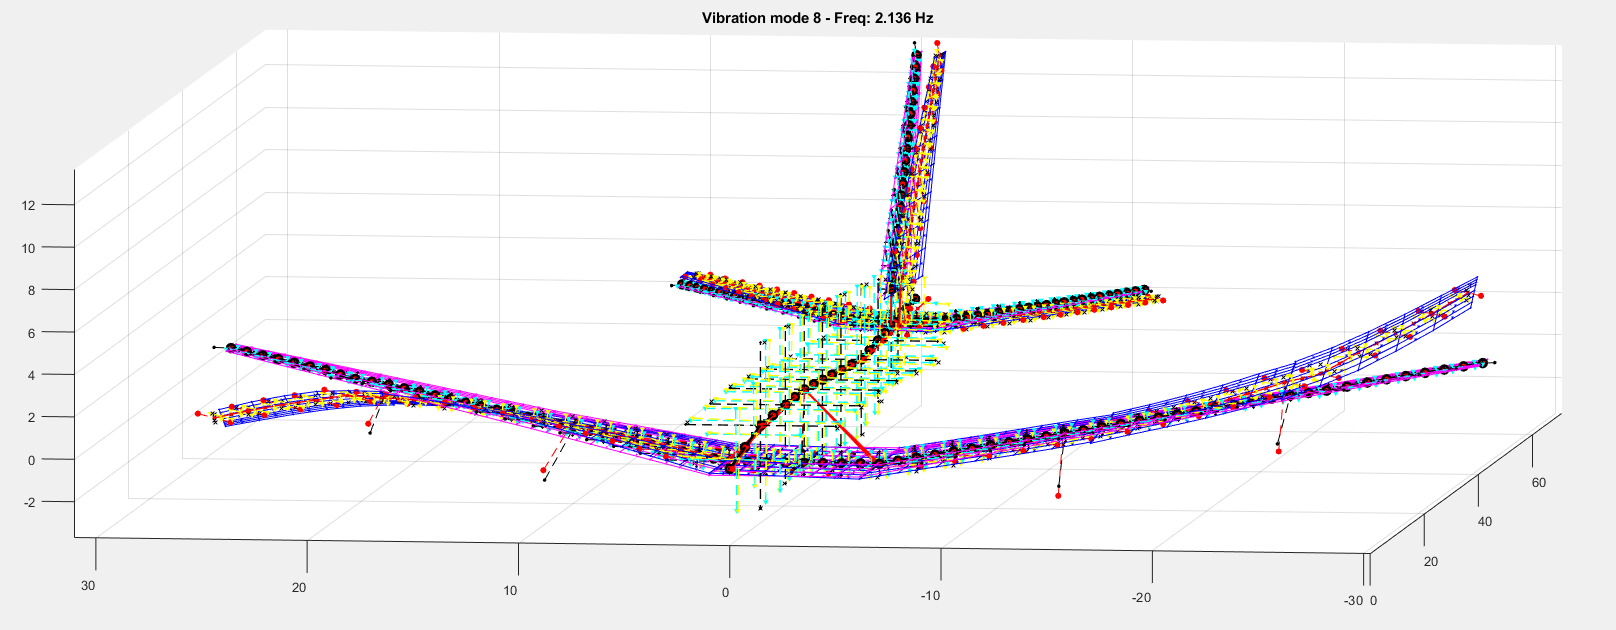
\includegraphics[width = 3in]{images/mode8-1e8.png}}\\
\caption{Modes 7 and 8 - $k_{hinge} = 1e8$}
\label{fig:modes7-8-1e8}
\end{figure*}

The comparison revealed that for low stiffnesses, the first non-rigid modes are clearly wingtip modes, but as the stiffness is increased, these modes tend to be more similar to the hingeless case modes.

All these results are consistent with previous works \cite{Castrichini2016, Wilson2014, Castrichini2020}.


\section{Flutter results}  
When flutter analysis is run in NeoCASS, V-f and V-g plots are obtained, where the evolution of both frequency and damping with velocity is shown for each mode considered. If at some point, the damping of one of the modes gets positive values, then flutter phenomenon appears. In figure \ref{fig:VgVf} an example of these plots is shown for the case when the hinge is located at 78\% of the semi wing and the hinge stiffness is  $k_{hinge} = 1e5 [Nm/rad]$.

\begin{figure}[htp]
  \centering
  \setlength\figureheight{5cm}
  \setlength\figurewidth{6cm}
  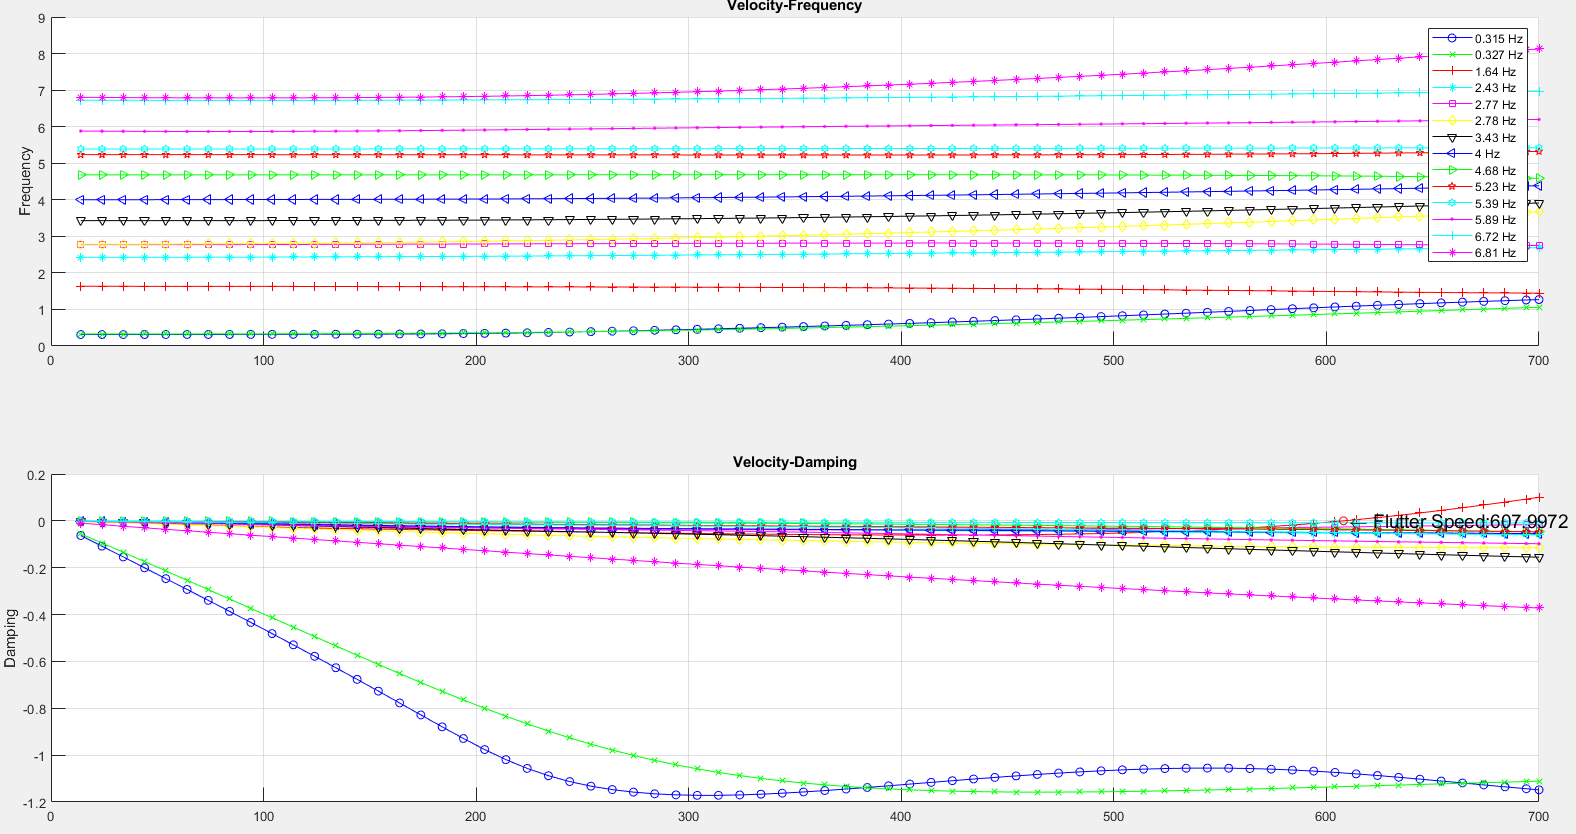
\includegraphics[width=250pt]{images/VgVf.png}
  \caption{V-f and V-g plots}
  \label{fig:VgVf}
\end{figure}

As described in \ref{sec:flutter-analysis}, this analysis was done for a large amount of hinge stiffness values in order to evaluate how this design parameter affects the flutter speed, i.e. the speed at which one of the modes gets positive values for its damping. Then, the procedure was repeated changing the location of the hinge.

Figure \ref{fig:flutter_total} group all the obtained results.

\begin{figure}[htp]
  \centering
  \setlength\figureheight{5cm}
  \setlength\figurewidth{6cm}
  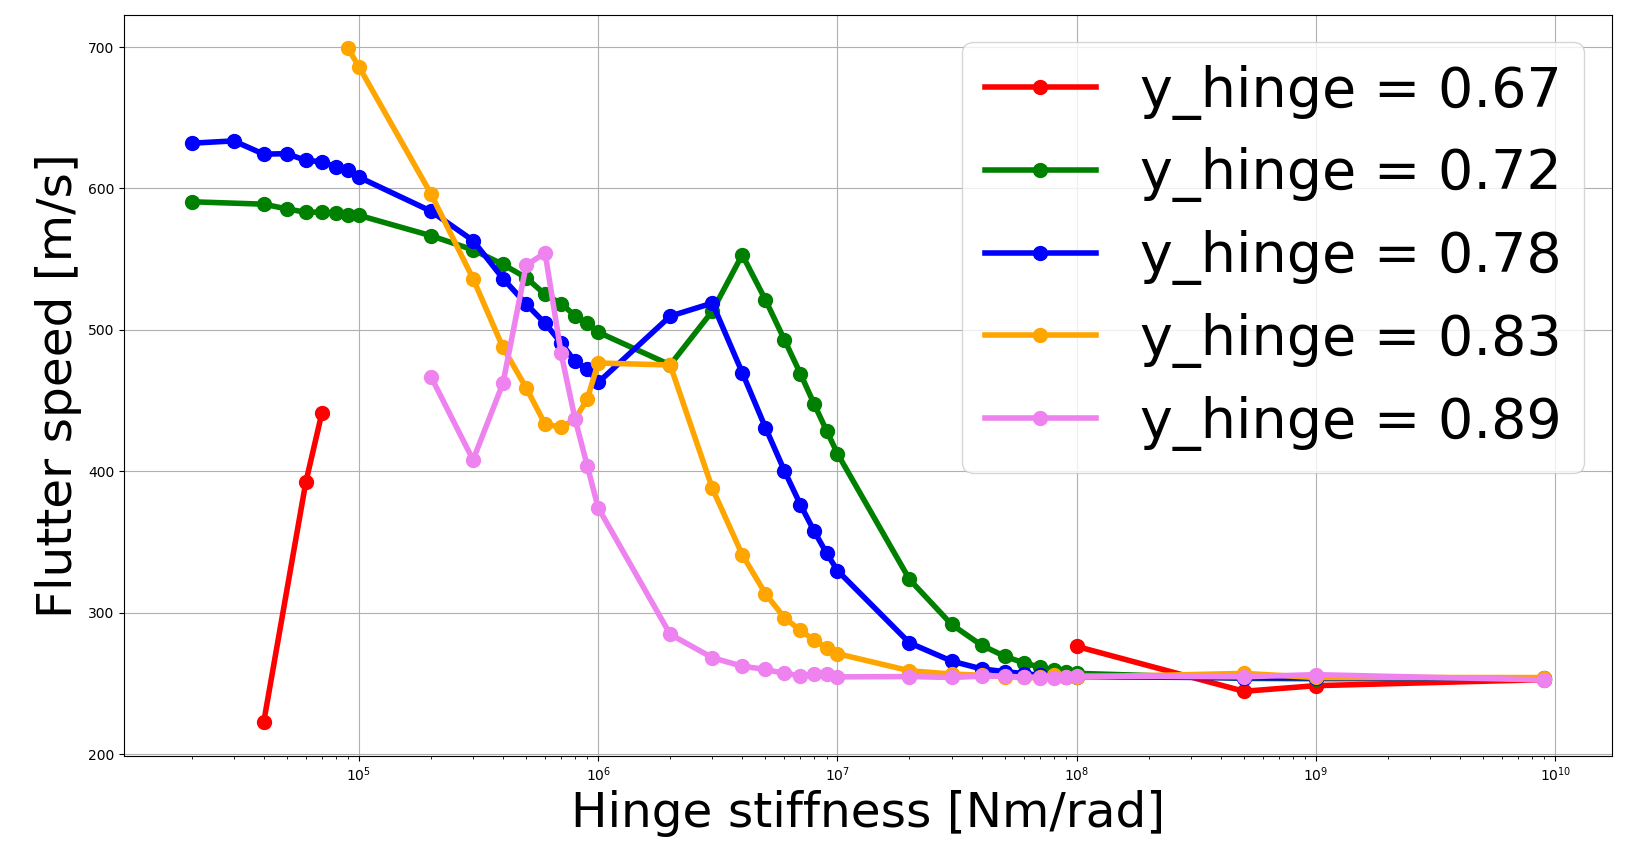
\includegraphics[width=250pt]{images/flutter_total.png}
  \caption{V-f and V-g plots}
  \label{fig:flutter_total}
\end{figure}

It is clear that, in general, lower stiffness values, produce higher flutter speeds, i.e. if the hinge stiffness is reduced, then a stabilising effect is generated. This can be explained by the fact that from a dynamic point, wingtip deflections introduced an aerodynamic damping contribution \cite{Castrichini2016}.

However, for hinge stiffness values lower than $k_{hinge} = 1e4 [Nm/rad]$, NeoCASS failed at finding convergence in the flutter analysis, which can be an indicator that strong instabilities appear when hinge stiffness is too low.

This effect is consistent with all values, except for a certain range between $k_{hinge} = 3e5 [Nm/rad]$ and $k_{hinge} = 4e6 [Nm/rad]$ approximately (depending on the hinge position), were the curves show a local maximum and if the stiffness keeps to be reduced, the flutter speed decreases. Out of this range, the flutter speed grows again as long as we reduce the hinge stiffness.

The described behaviour is due to a change in the mode that becomes unstable producing flutter. In figure \ref{fig:changeMode} this effect is highlighted for the case where the hinge is located at the 78\% of the semi wing. For high stiffness values, mode 11 becomes unstable generating flutter, whereas, for low stiffness values, mode 9 is the cause of the mentioned phenomenon.

\begin{figure}[htp]
  \centering
  \setlength\figureheight{5cm}
  \setlength\figurewidth{6cm}
  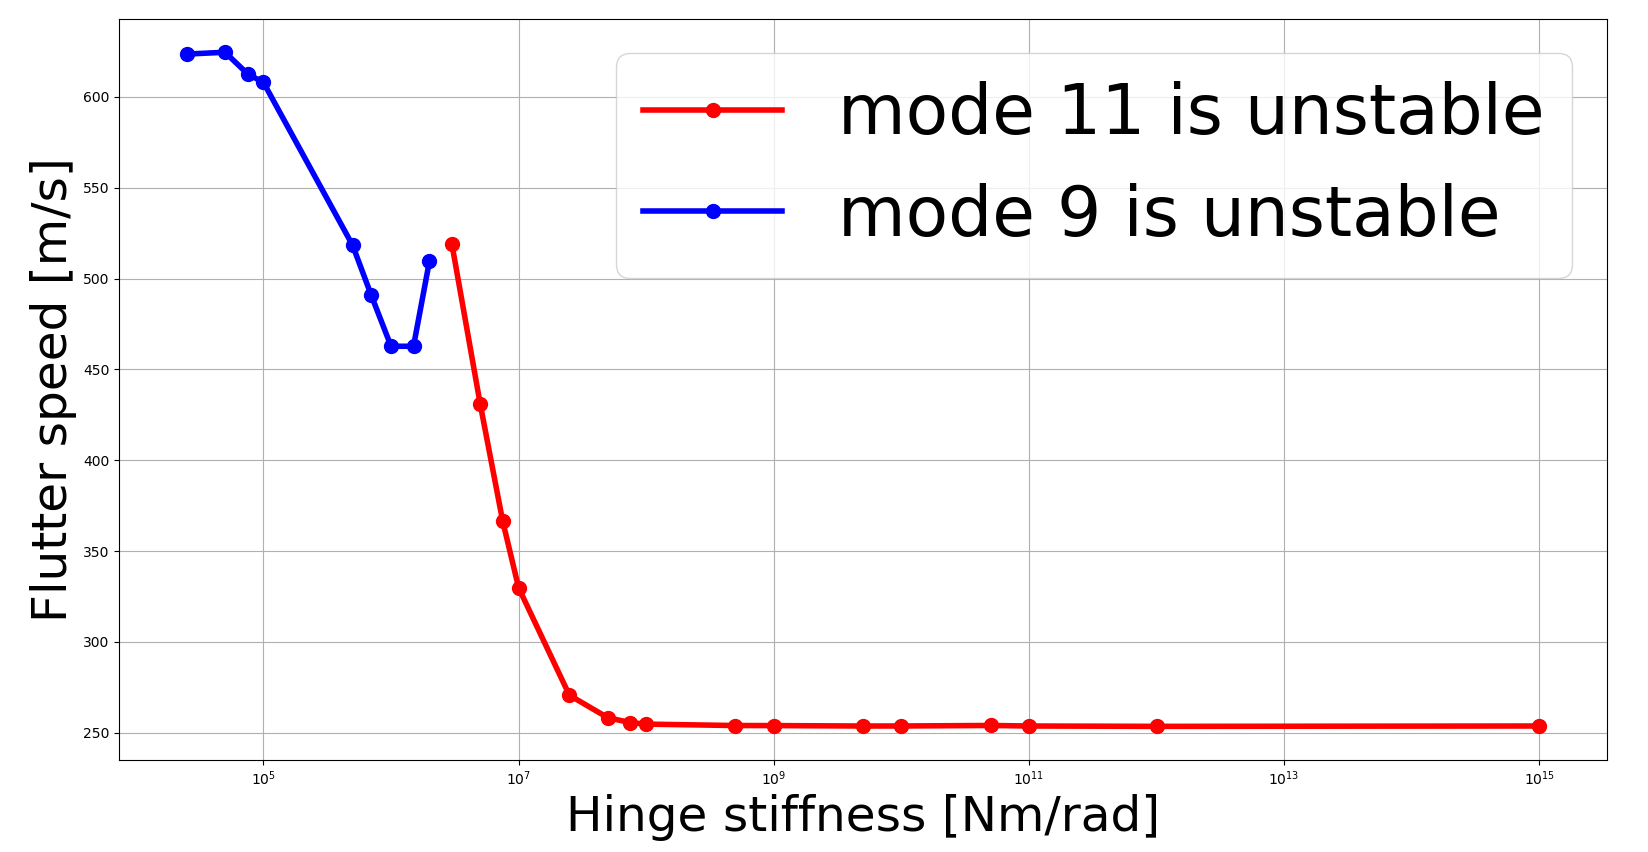
\includegraphics[width=250pt]{images/changeMode.png}
  \caption{Change in the unstable mode}
  \label{fig:changeMode}
\end{figure}

Concerning the hinge position influence, the results showed that moving the hinge inwards, i.e. towards the root of the wing, generates a strong stabilizing effect, increasing the flutter speed. In fact, for the case where the hinge is located at 67\% of the semi wing, there was no flutter for most of the hinge stiffness values.

Another significant point is that for stiffnesses greater than $k_{hinge} = 1e8 [Nm/rad]$ both hinge position and stiffness lose their influence. As is it shown in \ref{fig:flutter_total} flutter speed converge to a single value, in this case $V_f = 253.5 [m/s]$.


\section{Conclusions}

In this work, a new design solution was studied. A brief characterization of the context, including advantages and disadvantages, was done. Then, the techniques and procedures followed in order to model the hinge, as well as modal and flutter analysis configurations, were described.

Even if the model used is limited, significant qualitative results were obtained, indicating that both hinge position and stiffness can be used to control the aeroelastic stability of the aircraft.

The findings of this study indicate that locating the hinge closer to the wing root generates a stabilizing effect, increasing the flutter speed. The same effect is presented when the hinge stiffness is decreased. However, this last parameter has to be carefully selected since strong instabilities can be produced if the hinge stiffness is to low.


\section{Future work}
Future studies in the current topic are therefore required in order to achieve a better understanding of how the related phenomenons are influenced. Each step done is important to make this design solution closer to have practical applications in the future.

Improving the model would help to obtain quantitative results, for example, incorporating the flare angle as a design parameter, or working with high-fidelity models.

Also, the application of multidisciplinary design optimization can be useful when looking for a compromise between the effects generated by this kind of design.


% Optional section

\section*{Acknowledgment}
I would like to thank Dr Morlier for his support during the investigation and most of all for giving me the opportunity to work on this fascinating subject.

\bibliographystyle{plain}
\bibliography{references}

\end{document}


